\documentclass{template/openetcs_report}
% Use the option "nocc" if the document is not licensed under Creative Commons
%\documentclass[nocc]{template/openetcs_article} 
\usepackage{lipsum,url}
\usepackage{xspace}
\usepackage{graphicx}
\usepackage{fixme}
\usepackage{lscape} 
\usepackage{pgfgantt}
\usepackage{adjustbox}
\usepackage{datetime}
\usepackage{appendix}
\usepackage{enumerate}
\usepackage{tikz}
\usepackage{hyperref}
\usepackage{breakurl}
\usepackage{color, colortbl}
\definecolor{myblue}{rgb}{0.6,.6,1}
\definecolor{mydarkblue}{rgb}{0,0,0.5}
\definecolor{mylightblue}{rgb}{0.8,0.8,1}
\usetikzlibrary{arrows,shapes,automata,petri,calc}


%user specified macros
\newenvironment{activity}[2][planned]
	{\begin{tabular}{p{0.25\textwidth}@{\hspace{0.05\textwidth}}p{0.7\textwidth}}
			\multicolumn{2}{p{\textwidth}}{\colorbox{black}{\begin{minipage}{1.1cm}\begin{center}\textsc{\footnotesize \textcolor{white}{#1}}\end{center}\end{minipage}}~~\textbf{#2}}\\
	}
	{\end{tabular}}

\newcommand{\entry}[2]{#1:&#2\\}
\newcommand{\website}[1]{Website:&\url{#1}\\}
\newcommand{\desc}[1]{\multicolumn{2}{p{\textwidth}}{#1}\\}

\newcommand{\VV}{Verification \& Validation\xspace}
\newcommand{\vv}{verification \& validation\xspace}

\newcommand{\tbd}{\colorbox{cyan}{\%\%To Be Defined\%\%}}
\newcommand{\tbc}{\colorbox{cyan}{\%\%To Be Confirmed\%\%}}
\newcommand{\todo}[1]{\colorbox{cyan}{\%\%{#1}\%\%}}
\newcommand{\nthng}[1]{}
%% Requirements.


\newcounter{reqnum}
\setcounter{reqnum}{0}
\newcounter{subreqnum}
\newcounter{subsubreqnum}
\newlength{\partopbuf}
\newlength{\topbuf}

% Automated numbering versions of the macros
\newcommand{\req}[1]{\addtocounter{reqnum}{1} \setcounter{subreqnum}{0}
	\begin{description}\item[{\small\reqt-X-\thereqnum}] #1\end{description}
}

\newcommand{\subreq}[1]{
	\addtocounter{subreqnum}{1} \setcounter{subsubreqnum}{0}
	\addtolength{\leftmargini}{1cm}
	\begin{description}
	\item[\hspace{0.5cm}{\small\reqt-X-\thereqnum.\thesubreqnum}] #1
	\end{description}
	\addtolength{\leftmargini}{-1cm}
}

\newcommand{\subsubreq}[1]{
	\addtocounter{subsubreqnum}{1}
	\addtolength{\leftmargini}{2cm}
	\begin{description}
	\item[\hspace{1cm}{\small\reqt-X-\thereqnum.\thesubreqnum.\thesubsubreqnum}] #1
	\end{description}
	\addtolength{\leftmargini}{-2cm}
}

% Fixed version of the commands
\newcommand{\reqfixed}[3]{\addtocounter{reqnum}{1} \setcounter{subreqnum}{0}
	\begin{description}\item[{\small\reqt-#1-#2}] #3\end{description}
}

\newcommand{\subreqfixed}[4]{
	\addtocounter{subreqnum}{1} \setcounter{subsubreqnum}{0}
	\addtolength{\leftmargini}{1cm}
	\begin{description}
	\item[\hspace{0.5cm}{\small\reqt-#1-#2.#3}] #4
	\end{description}
	\addtolength{\leftmargini}{-1cm}	
}

\newcommand{\subsubreqfixed}[5]{
	\addtocounter{subsubreqnum}{1}
	\addtolength{\leftmargini}{2cm}
	\begin{description}
	\item[\hspace{1cm}{\small\reqt-#1-#2.#3.#4}] #5
	\end{description}
	\addtolength{\leftmargini}{-2cm}	
}

% Citation of the requirement

% Citation of the reference (for markup purpose)
%\newcommand{\refreq}[1]{\textbf{#1}}

% Citation of the reference and text (for markup purpose)
% The purpose of this is to automatically replace the placeholder by the 
% full text. \fullrefreq{R-xxx}{} or \fullrefreq{R-xxx}{blabla} 
% will be replaced by \fullrefreq{R-xxx}{text of the R-xxx requirement} 
%\newcommand{\fullrefreq}[2]{\textbf{#1}: \textrm{#2}}

\def\reqt{R-WP2/D2.6}
\newenvironment{justif}{
	\begin{quote}
	\begin{itshape}Justification. 
}{
	\end{itshape}
	\end{quote}
}
%Uncertain items
\newcommand{\qq}[1]{?`#1?}
%C++
\newcommand{\cxx}{C\nolinebreak[4]\hspace{-.05em}\raisebox{.3ex}{\footnotesize\bf ++}\xspace}

\renewcommand{\tbd}[1]{\nthng{#1}}


\graphicspath{{./template/}{.}{./images/}}
\begin{document}
\frontmatter
\project{openETCS}

%Please do not change anything above this line
%============================
% The document metadata is defined below

%assign a report number here
\reportnum{OETCS/WP3/D3.6.1.1}

%define your workpackage here
\wp{Work Package 1: ``Governance''}

%set a title here
\title{openETCS Software Release and Deployment Plan}

%set a subtitle here
\subtitle{Version 0.1.0}

%set the date of the report here
\date{06. May 2014}

%define a list of authors and their affiliation here

\author{
Bernd Hekele (DB-Netz AG)\\
\small
{\it Contributions by:} \\}

\affiliation{DB-Netz AG\\
  V\"olckerstrasse 5\\
  80939 M\"unchen,   Germany
   \\eMail:bernd.hekele@deutschebahn.com }
  
% define the coverart
\coverart[width=350pt]{openETCS_EUPL}

%define the type of report
\reporttype{Part of Quality Assurance Plan}



\begin{abstract}
%define an abstract here

This document describes the strategy and plan of software releases in the openETCS ITEA project.


\end{abstract}

%=============================
%Do not change the next three lines
\maketitle
\tableofcontents
\listoffiguresandtables
\newpage
%=============================

\chapter{Document Control}

\begin{tabular}{|p{4.4cm}|p{8.7cm}|}
  \hline
  \multicolumn{2}{|c|}{Document information} \\
  \hline
  Work Package &  WP1  \\
  Deliverable ID or doc.\ ref.\ & D1.3.1\\
  \hline
  Document title & openETCS Software Release and Deployment Plan\\
  Document version & 0.1.0 \\
  Document authors (org.)  &  Bernd Hekele (DB-Netz AG)\\
  \hline
\end{tabular}

\begin{tabular}{|p{4.4cm}|p{8.7cm}|}
\hline
\multicolumn{2}{|c|}{Review information} \\
\hline
Last version reviewed & -- \\
\hline
Main reviewers & -- \\
\hline
\end{tabular}

\begin{tabular}{|p{2.2cm}|p{4cm}|p{4cm}|p{2cm}|}
\hline
\multicolumn{4}{|c|}{Approbation} \\
\hline
  &  Name & Role & Date   \\
\hline  
Written by    &  Bernd Hekele & WP3 Task 3.6 Leader  & May 2014\\
\hline
Approved by &  &  &  \\
\hline
\end{tabular}

\begin{tabular}{|p{1.5cm}|p{2cm}|p{3.5cm}|p{6cm}|}
\hline
\multicolumn{4}{|c|}{Document evolution} \\
\hline
Version &  Date & Author(s) & Comment  \\
\hline  
00.01 & 17.04.2014 & Bernd Hekele &  Document creation
\\\hline  
00.01 & 06.05.2014 & Bernd Hekele &  First comments on Structure included
\\\hline
\end{tabular}

% The actual document starts below this line
%=============================


%Start here

\mainmatter

\chapter{Introduction}
From its nature openETCS is not a simple development project. In openETCS other aspects have a similar weight compared to the actual developed product:
\begin{itemize}
\item Clarification of the SRS, Clearing of Findings.
\item Introduction of a formal model to be used as a quasi standard extension for the SRS
\item Introduction of Agile Methods in Development.
\item Introduction of openSource and openProofs as a method to produce safety critical software.
\item Production of a software build to show the standard alive in a ETCS demonstrator.
\end{itemize} 
These additional tasks are part of the research character of the openETCS project.\\
These research aspects have an implication on this release plan as well:
\begin{enumerate}
\item We do not plan to deliver a safe product to run a train. 
\item We do not start with fixed processes at the beginning of the project. Processes are developed hand-in-hand with the progress of the development work.
\item We have some additional outputs as a result of the release which are not common to this class of development.
\end{enumerate}

This document (the plan) also will be developed further with each iteration in the project. An updated and enriched version is planned:
\begin{enumerate}
\item At the end of the first iteration\\
This update will define deliverables of regular iteration releases in detail:
\begin {itemize}
\item When do we release?
\item Where do we release?
\item What do we release?
\item In which quality do we release?\\
Mandatory Checks
\item Procedures to report findings of iteration releases.
\end{itemize}

\item At the end of the each following iteration\\
We will incorporate our lessons learned and findings of the Scrum Rehearsal. 
\end{enumerate}

\section{openETCS Release Stakeholders}

Unlike other development projects the modelling result (i.e., the content of the releases) is not directly feeding into a product. But, we have to support our internal stakeholders for the modelling results:
\begin{itemize}
\item Verification \& Validation (WP4).
\item Demonstrator (WP5), i.e., the code goes directly into a train simulator.
\item The Railway Community (represented by ERA), who especially is interested in the clarification of the standards.

\end{itemize}


\section{Glossary}
\label{sec:glossary}

\begin{description}
\item[API:] Application Programming Interface. In the project, the API defines 
the interface of the EVC software to the operating system and hardware. \textit{The
exact nature of the API still needs to be defined, whether it should be seen as
a specification or as an implementation has yet to be resolved.}
\item[Build:] A compiled package of software. If possible, the package will be integrated in a binary ready for testing. Builds can be produced frequently to support the integration of software parts [daily Build]. In openETCS a build has to be produced at least at the end of a sprint.
\item[Deployment:]
\item[Release:] A release is a build with a qualified status by verification and validation.
\item[Iteration:] A number of sprints defined to reach a defined scope of the model. In openETCS we plan to have a release at the end of an iteration.
\item[Sprint:] Phase in agile development. See Definition of Scrum in the QA-Plan. In openETCS modelling, the sprint lasts 2 weeks. At the end of a sprint, the artefacts will be produced in a sprint build. To get the stamp "Done" the function of artefacts have to be demonstrated in the sprint review meeting.
\item[SRS:] (ERTMS/ETCS-) System Requirements Specification. 
\item[SW:] Software

\chapter{The Release Plan}

\section{The Release Template}
For documentation of releases a template is to be used. You can find the template in this location: \url{https://github.com/openETCS/governance/blob/master/SoftwareReleaseAndDeploymentPlan/openETCSReleaseTemplate.tex}.

\section{openETCS Timeline: Development Phases}

\begin{figure}
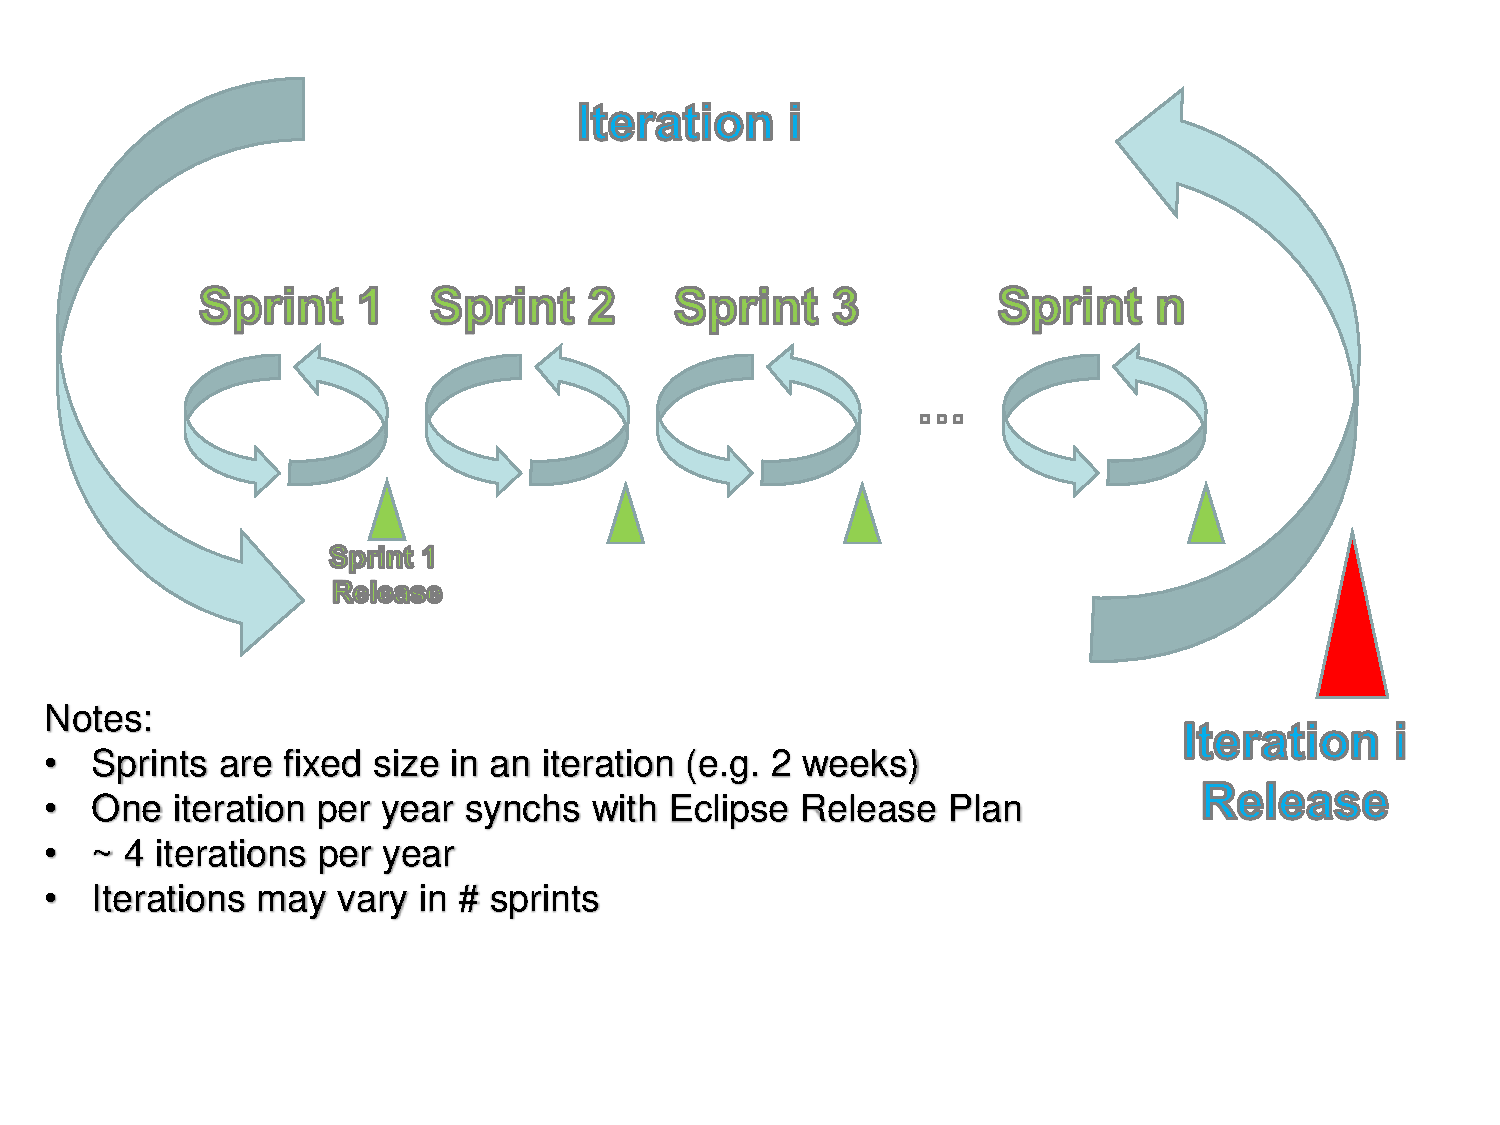
\includegraphics[width=\textwidth]{figures/iterations.pdf}
\caption{Sprints, Iterations and Releases
\label{f:iteration}}
\end{figure}

openETCS modelling introduces agile development methods. Basis for a release plan in an agile world is visible in the following planning concepts (please, refer to figure \ref{f:iteration}). The figure shows the tools in openETCS and artefacts needed as input our output from the tools. In ´general, all results from the production process are provided as a part of releases, e.g., generated code, compilation listings, object code etc.

\begin{itemize}
\item \textbf{Sprint}\\
An openETCS modelling sprint is planned to last for 2 weeks. During the sprint a team works on priorized items taken from the modelling backlog. Each item has a "Done" criteria to be reached at the end of the sprint. The "done" criteria is the target for validation which is done as a part of the sprint. To support agile we need some principles:
\item \textbf{Daily Builds}\\
 during the Sprint. The daily build has to integrate all software parts of openETCS modelling. The concept for openETCS has to be elaborateds and will be started as soon as sufficient code has been generated and integrated (second iteration).
\item \textbf{Automated Tests}\\
 for validation of the daily build and - more important - at the end of the sprint for the sprint review.
\item \textbf{A sprint release} for each successfully completed sprint.
\item \textbf{Iteration}\\
The openETCS modelling will increase the coverage of the SRS functionality in iterations. The duration of an itreration is defined by the number of sprints planned for the iteration. The content of the iteration will be defined at the end of the previous iteration and is visible in the srs-analysis issues tracker:
\url{https://github.com/openETCS/srs-analysis/issues/milestones}. Iterations do not have a fixed length, however, we shall plan for about 4 iterations per year. Each iteration has an iteration release as a result. The release might be taken by WP5 for building a new version of the openETCS demonstrator.
\item \textbf{First Iteration}\\
The first Iteration is defined with a strictly limited scope in order to run the full modelling cycle and producing the full set of artefacts in onpenETCS. Target of the iteration is the proof of the concept in a small model.
\item \textbf{Second Iteration}\\
The second iteration shall be defined from an operational point of view. The scenario shall cover - under well defined operational limitations - all functions needed to start the train, control speed and stop the train. Details will be defined in an openETCS modelling workshop based on the recommendation of the openETCS stakeholders (WP4, WP5, operators).

\item \textbf{Release in the context of Eclipse}\\
Each year the Eclipse Foundation produce a release on a coordinated schedule:\\
\url{http://wiki.eclipse.org/Simultaneous_Release}\\
openETCS will synchronise a yearly release with the Eclipse schedule. The openETCS release covers toolchain as well as modelling results. In modelling, a convenient iteration will be chosen for this approach.\\
   
\end{itemize}

Setting for the first iteration: 6 sprints, each sprint 2 weeks.\\
Proposed setting for the second iteration: 10 sprints, each sprint 2 weeks.\\


\section{openETCS Scope of the Release}

\begin{figure}
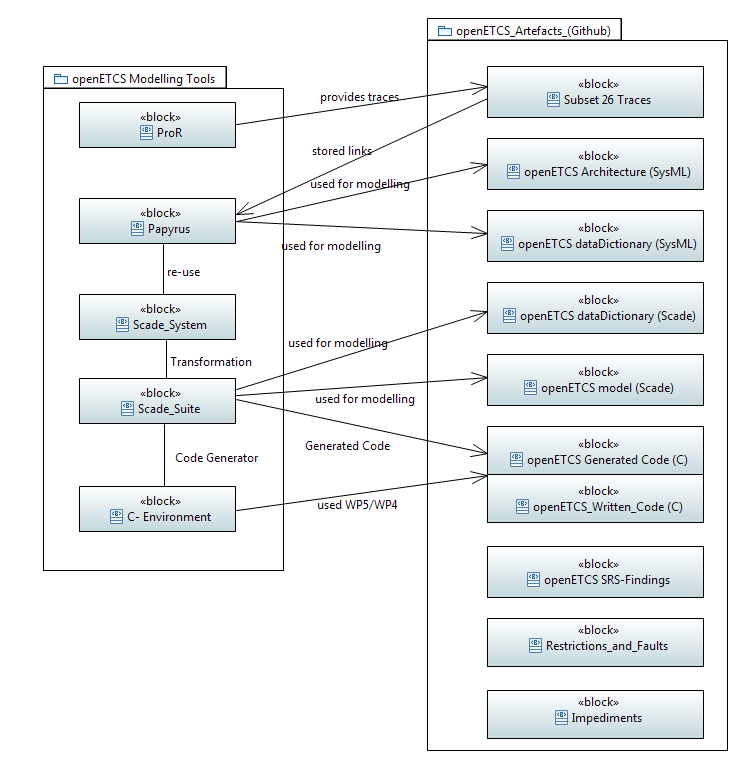
\includegraphics[width=\textwidth]{figures/ReleasePlan.png}
\caption{openETCS Tools and Artefacts
\label{f:tools}}
\end{figure}

In this section, we define the scope and the quality of the openETCS modelling releases according to the use-case. Links to the location in the openETCS repositories will be provided as soon as they are defined.
Figure \ref{f:tools} indicates the artefacts and the respective use-case. The current diagram is limited to modelling.


\begin{itemize}
\item \textbf{Daily Build Report}\\
The Build Report, i.e., details of the server are to be clarified. At the server, the following information is available:

\begin{enumerate}
\item Build Highlights (Entry Page on wiki with summary information)
\item Information on which version of model parts have been used to make the build.
\item Generated C-Code
\item Generation Result (Scade Suite Output)
\item Compilation Result and Object Code
\item Test results of automated test-cases 
\end{enumerate}

\item \textbf{Sprint Release Report}\\
The sprint release, i.e., details related to the sprint result:
\begin{enumerate}
\item Build Report of final build of the sprint
\item Updated SysML model, Synchronisation of Scade Suite and Scade System model 
\item Updated Sprint Backlog incl. "Done" Status of items
\item Restrictions and Fault reports related to failed backlog items
\item List of Impediments
\end{enumerate}

\item \textbf{Iteration Release Report}
\begin{enumerate}
\item Sprint Release Report of last Sprint of the Iteration
\item Sprint Retrospective Result
\item The SysML and the Scade Suite model
\item validation results
\item List of open Errors and Restrictions (with Status and Priority)
\item Update on SRS Findings
\end{enumerate}

\item \textbf{Yearly Eclipse Synchronised Release}
\begin{enumerate}
\item Iteration Release Report of relevant iteration
\item update of project status
\end{enumerate}

\end{itemize}

\chapter{The Deployment Plan}

In this project, deployment covers the delivery of a release to the demonstrator work package. The openETCS model is part of the simulation framework - not of a real train. Since openETCS follows the Eclipse philosophy a yearly release of the openETCS model e.g., synchronised with the Eclipse coordinated releases, is planned. 

The plan relevant for deployment will be available at the end of the second iteration.
The plan will answer the questions:
\begin {itemize}
\item When do we deploy?
\item Where do we deploy?
\item What do we deploy?
\item In which quality do we deploy?
\item Procedures to report findings.
\end{itemize}
\end{description}

\chapter{References}
\begin{itemize}
\item \textbf{D1.3.1}: Quality Assurance Plan
\item \textbf{D1.3.1}: Software Release Template
\end{itemize}

\bibliographystyle{unsrt}
\bibliography{bibliography}


\nocite{*}
%===================================================
%Do NOT change anything below this line

\end{document}
